\documentclass{../../../oss-classkick-exam}

\begin{document}
\genheader

\gentitle{C}{CICULAR MOTION}

\genmultidirections

\gengravity

\raggedcolumns
\begin{multicols*}{2}
  \begin{questions}
    \question A girl stands on a rotating merry-go-round without holding on to
    a rail. The force that keeps her moving in a circle is the
    \begin{choices}
      \choice frictional force on the girl directed away from the center of the
      merry-go-round
      \choice frictional force on the girl directed toward the center of the
      merry-go-round
      \choice normal force on the girl directed away from the center of the
      merry-go-round
      \choice normal force on the girl directed toward the center of the
      merry-go-round
      \choice weight of the girl
    \end{choices}
    \vspace{.7in}
    
    % This problem needs some fixing. None of the answers are correct
%  \item A \SI{.5}{\kilo\gram} ball on the end of a \SI{.5}{\metre} long string
%    is swung in a horizontal circle. What would the speed of the ball have to
%    be for the tension in the string to be \SI{9.}{\newton}?
%    \begin{choices}
%    \choices\SI{1}{\metre\per\second}
%    \choices\SI{3}{\metre\per\second}
%    \choices\SI{6}{\metre\per\second}
%    \choices\SI{9}{\metre\per\second}
%    \choices\SI{12}{\metre\per\second}
%    \end{choices}

    \uplevel{
      \begin{center}
        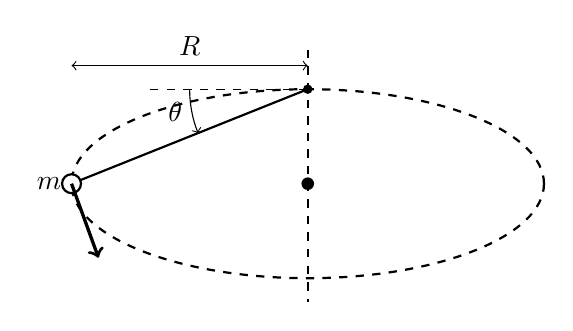
\begin{tikzpicture}
          \fill(0,0) circle(.08);
          \fill(0,1.2)circle(.06);
          \draw[thick,dashed](0,0) ellipse(3 and 1.2);
          \draw[thick,dashed](0,1.7)--(0,-1.5);
          \draw[thick](-3,0)--(0,1.2);
          \draw[thick,fill=white](-3,0) circle(.12) node[left]{$m$};
          \draw[<->](0,1.5)--(-3,1.5) node[midway,above]{$R$};
          \draw[dashed](0,1.2)--(-2,1.2);
          \draw[->](-1.5,1.2) arc(180:202:1.5) node[midway,left]{$\theta$};
          \draw[very thick,->,rotate around={20:(-3,0)}](-3,0)--(-3,-1)
          node[below]{$\varv$};
        \end{tikzpicture}
      \end{center}

      \textbf{Questions \ref{ball1}--\ref{ball2}}

      A ball of mass $m$ and weight $W$ on the end of a string is swung in a
      horizontal circle of radius $R$ with a speed $\varv$. The string makes an
      angle $\theta$ below the horizontal, as shown. The magnitude of the
      tension in the string is $T$.
    }


  \question Which of the following diagrams best shows the forces acting on the
    ball as it moves in a circle? 
    \begin{choices}
      \choice
      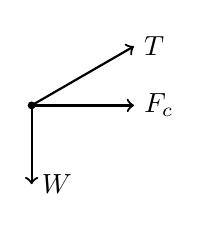
\begin{tikzpicture}
        \fill(0,0) circle(.05);
        \begin{scope}[thick,->]
          \draw (0,0)--(0,-1)node[right]{$W$};
          \draw (0,0)--(1.3,0) node[right]{$F_c$};
          \draw[rotate=30] (0,0)--(1.5,0) node[right]{$T$};
      \end{scope}
      \end{tikzpicture}
      
      \choice
      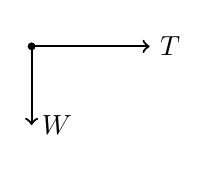
\begin{tikzpicture}
        \fill(0,0) circle(.05);
        \begin{scope}[thick,->]
          \draw (0,0)--(0,-1)node[right]{$W$};
          \draw (0,0)--(1.5,0) node[right]{$T$};
        \end{scope}
      \end{tikzpicture}
      
      \choice
      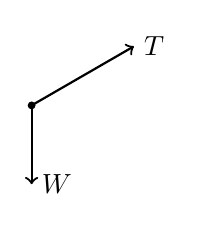
\begin{tikzpicture}
        \fill(0,0) circle(.05);
        \begin{scope}[thick,->]
          \draw (0,0)--(0,-1)node[right]{$W$};
          \draw[rotate=30] (0,0)--(1.5,0) node[right]{$T$};
        \end{scope}
      \end{tikzpicture}

      \choice
      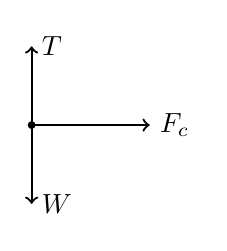
\begin{tikzpicture}
        \fill(0,0) circle(.05);
        \begin{scope}[thick,->]
          \draw (0,0)--(0,-1)node[right]{$W$};
          \draw (0,0)--(1.5,0) node[right]{$F_c$};
          \draw (0,0)--(0,1) node[right]{$T$};
        \end{scope}
      \end{tikzpicture}
      
      \choice
      \begin{tikzpicture}
        \fill(0,0) circle(.05);
        \begin{scope}[thick,->]
          \draw (0,0)--(0,-1)node[right]{$W$};
          \draw[rotate=120] (0,0)--(1.5,0) node[left]{$T$};
        \end{scope}
      \end{tikzpicture}
    \end{choices}
    \label{ball1}
    
    \question In terms of $m$, $R$, $\varv$, and $\theta$, the magnitude of the
    tension $T$ is
    \begin{choices}
      \choice $\dfrac{m\varv^2}R$
      \choice $\dfrac{m\varv^2}{R\sin\theta}$
      \choice $\dfrac{m\varv^2}{R\cos\theta}$
      \choice $\dfrac{m\varv}{R\sin\theta}$
      \choice $m\varv R\sin\theta$
    \end{choices}
    \label{ball2}
    \columnbreak
    
  \question A ball of mass $m$ is swung in a vertical circle of radius $R$. The
    speed of the ball at the bottom of the circle is $\varv$. The tension in the
    string at the bottom of the circle is
    \begin{choices}
      \choice $mg$
      \choice $mg+\dfrac{m\varv^2}{R}$
      \choice $mg-\dfrac{m\varv^2}{R}$
      \choice $\dfrac{m\varv^2}{R}$
      \choice 0
    \end{choices}
    
  \question A car of mass $m$ drives on a flat circular track of radius $R$. To
    maintain a constant speed $\varv$ on the track, the coefficient of friction
    $\mu$ between the tires and the road must be
    \begin{choices}
      \choice $mg$
      \choice $mg+\dfrac{m\varv^2}{R}$
      \choice $mg-\dfrac{m\varv^2}{R}$
      \choice $\dfrac{\varv^2}{gR}$
      \choice $\sqrt{\dfrac{\varv^2}{gR}}$
    \end{choices}

    \uplevel{
      \textbf{Questions \ref{rad1}--\ref{rad2}}
    }

  \question A ball on the end of a string is swung in a circle of radius
    \SI{2}{\metre} according to the equation $\theta = 4t^2+3t$, where $\theta$
    is in radians and $t$ is in seconds. The angular acceleration of the ball
    is
    \begin{choices}
      \choice\SI{6}{rad\per\second\squared}
      \choice $4t^2 + 3t$ \si{rad\per\second\squared}
      \choice $8t +3$ \si{rad\per\second\squared}
      \choice $\displaystyle\frac{3}{4} t^3 + 3t^2$ \si{rad\per\second\squared}
      \choice \SI{8}{rad\per\second\squared}
    \end{choices}
    \label{rad1}
    
  \question The linear speed $v$ of the ball at $t=\SI3\second$ is
    \begin{choices}
      \choice \SI{27 }{\metre\per\second}
      \choice \SI{54 }{\metre\per\second}
      \choice \SI{108}{\metre\per\second}
      \choice \SI{135}{\metre\per\second}
      \choice \SI{210}{\metre\per\second}
    \end{choices}
    \label{rad2}
    
%  \question Two wheels are attached to each other and fixed so that they can only
%    turn together. The smaller wheel has a radius of $r$ and the larger wheel
%    has a radius of $3r$. The two wheels can rotate together on a frictionless
%    axle. Three forces act tangentially on the edge of the wheels as shown.
%    The magnitude of the net torque acting on the system of wheels is
%    \begin{center}
%      \pic{.25}{2wheels.png}
%    \end{center}
%    \begin{choices}
%    \choices$Fr$
%    \choices$2Fr$
%    \choices$3Fr$
%    \choices$4Fr$
%    \choices$6Fr$
%    \end{choices}
%    \columnbreak
    
  \question A belt is wrapped around two wheels as shown. The smaller wheel has
    a radius $r$, and the larger wheel has a radius $2r$. When the wheels turn,
    the belt does not slip on the wheels, and gives the smaller wheel an
    angular speed $\omega$. The angular speed of the larger wheel is
    \cpic{.3}{wheels}
    \begin{choices}
      \choice $\dfrac14\omega$
      \choice $\dfrac12\omega$
      \choice $\omega$
      \choice $2\omega$
      \choice $4\omega$
    \end{choices}
    \columnbreak

    \uplevel{
      \begin{center}
        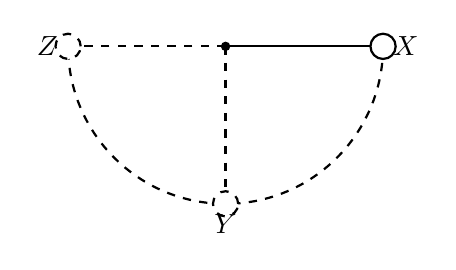
\begin{tikzpicture}[scale=2]
          \draw[dashed,thick](1,0) arc(0:-180:1);
          \draw[thick](0,0)--(1,0);
          \draw[thick,fill=white](1,0) circle(.08) node[right]{$X$};
          \draw[dashed,thick](0,0)--(-1,0);
          \draw[dashed,thick,fill=white](-1,0) circle(.08) node[left]{$Z$};
          \draw[dashed,thick](0,0)--(0,-1);
          \draw[dashed,thick,fill=white](0,-1) circle(.08) node[below]{$Y$};
          \fill(0,0) circle(.03);
        \end{tikzpicture}
      \end{center}
    }

  \question A ball on the end of a string is released from rest at point $X$ as
    shown. The ball swings under the influence of gravity from point $X$ through
    points $Y$ and $Z$. What are the directions of the acceleration vectors at
    points $Y$ and $Z$, respectively?
    \begin{tabular}{cll}
      (A) & Point $Y$: {\LARGE $\uparrow$} & Point $Z$: {\LARGE $\leftarrow$}\\
      (B) & Point $Y$: {\LARGE $\downarrow$}& Point $Z$: {\LARGE $\downarrow$}\\
      (C) & Point $Y$: {\LARGE $\nwarrow$} & Point $Z$: {\LARGE $\searrow$}\\
      (D) & Point $Y$: {\LARGE $\searrow$} & Point $Z$: {\LARGE $\leftarrow$}\\
      (E) & Point $Y$: {\LARGE $\downarrow$} & Point $Z$: {\LARGE $\searrow$}\\
    \end{tabular}
    \vspace{.7in}
    
  \question A merry-go-round is initially at rest, and begins to rotate with a
    constant angular acceleration $\alpha$. The angular speed $\omega$ of the
    merry-go-round after making two complete revolutions is
    \begin{choices}
      \choice $2\alpha$
      \choice $4\alpha$
      \choice $\sqrt{2\pi\alpha}$
      \choice $4\pi\alpha$
      \choice $\sqrt{8\pi\alpha}$
    \end{choices}

    \uplevel{\begin{center}
        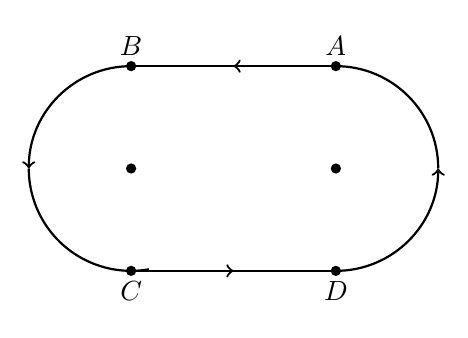
\begin{tikzpicture}[scale=1.3]
          \begin{scope}[thick]
            \draw[->](0,0) arc(-90:0:1);
            \draw (1,1) arc(0:90:1);
            \draw[->](0,2)--(-1,2);
            \draw(0,2)--(-2,2);
            \draw[->](-2,2) arc(90:180:1);
            \draw (-3,1) arc(180:280:1);
            \draw[->](-2,0)--(-1,0);
            \draw(-2,0)--(0,0);
            \fill( 0,0) circle(.05) node[below]{$D$};
            \fill( 0,2) circle(.05) node[above]{$A$};
            \fill(-2,2) circle(.05) node[above]{$B$};
            \fill(-2,0) circle(.05) node[below]{$C$};
            \fill(-2,1) circle(.05);
            \fill( 0,1) circle(.05);
          \end{scope}
        \end{tikzpicture}
      \end{center}
    }

    \question A speed skater races around a track in which the sides are equal
    length and parallel and the curves are semicircular. The skater keeps a
    constant speed throughout one entire lap. She starts at point $A$ and
    travels counterclockwise around the track for one lap. Which of the
    following graphs best represents the magnitude of the skater's acceleration
    as a function of time for one lap?
    \begin{choices}
      \choice
      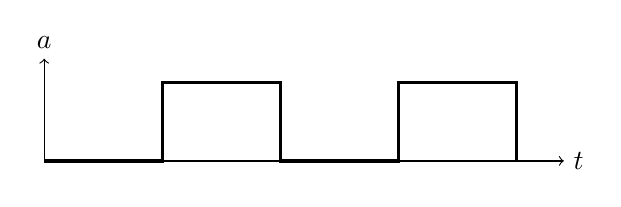
\begin{tikzpicture}
        \draw[->](0,0)--(6.6,0) node[right]{$t$};
        \draw[->](0,0)--(0,1.3) node[above]{$a$};
        \draw[very thick](0,0)--(1.5,0)--(1.5,1)--(3,1)--(3,0)--(4.5,0)--(4.5,1)
        --(6,1)--(6,0);
      \end{tikzpicture}

      \choice
      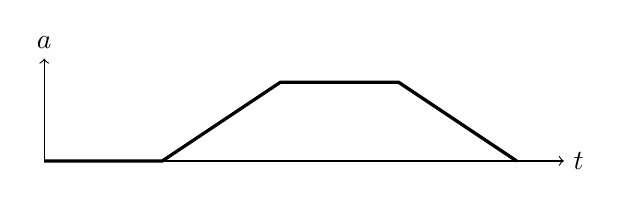
\begin{tikzpicture}
        \draw[->](0,0)--(6.6,0) node[right]{$t$};
        \draw[->](0,0)--(0,1.3) node[above]{$a$};
        \draw[very thick](0,0)--(1.5,0)--(3,1)--(4.5,1)--(6,0);
      \end{tikzpicture}

      \choice
      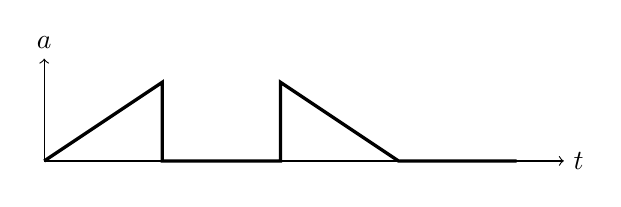
\begin{tikzpicture}
        \draw[->](0,0)--(6.6,0) node[right]{$t$};
        \draw[->](0,0)--(0,1.3) node[above]{$a$};
        \draw[very thick](0,0)--(1.5,1)--(1.5,0)--(3,0)--(3,1)--(4.5,0)--(6,0);
      \end{tikzpicture}

      \choice
      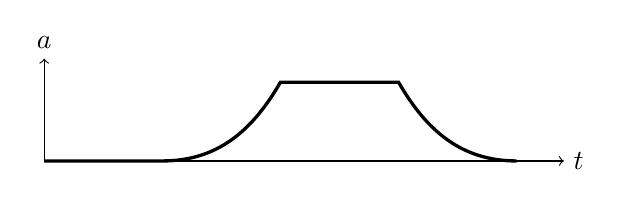
\begin{tikzpicture}
        \draw[->](0,0)--(6.6,0) node[right]{$t$};
        \draw[->](0,0)--(0,1.3) node[above]{$a$};
        \draw[very thick](0,0)--(1.5,0) to[out=0,in=240] (3,1)--(4.5,1)
        to [out=-60,in=180] (6,0);
      \end{tikzpicture}
     
      \choice
      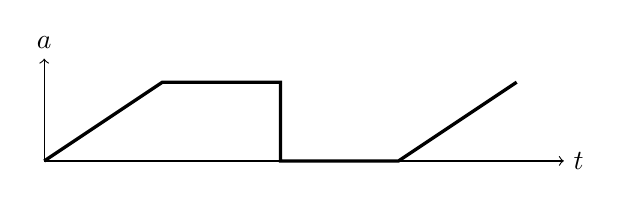
\begin{tikzpicture}
        \draw[->](0,0)--(6.6,0) node[right]{$t$};
        \draw[->](0,0)--(0,1.3) node[above]{$a$};
        \draw[very thick](0,0)--(1.5,1)--(3,1)--(3,0)--(4.5,0)--(6,1);
      \end{tikzpicture}
    \end{choices}

    \uplevel{
      \cpic{.18}{amusement}
    }
    
  \question An amusement park ride consists of a cylindrical room that spins so
    that people leaning up against the wall can stick to the wall even if the
    floor is lowered out from under them. The rotating room reaches a maximum
    angular speed $\omega$, the floor is lowered, and the riders stick to
    the wall. Which of the following statements is true?
    \begin{choices}
      \choice The weight of each rider provides the centripetal force keeping
      the rider moving in a circle.
      \choice The normal force applied by the wall must equal the weight of the
      rider.
      \choice The difference between the normal force applied by the wall and
      the weight of the rider is equal to the centripetal force acting on the
      rider.
      \choice The frictional force between the wall and the rider must equal the
      weight of the rider.
      \choice The frictional force between the wall and the rider provides the
      centripetal force acting on the rider.
    \end{choices}
    \vspace{.7in}

    \uplevel{  
      \begin{center}
        \begin{tikzpicture}[scale=.8]
          \draw[thick](-2,0)--(2,0);
          \draw[thick](0,-2)--(0,2);
          \draw[thick,fill=white](-2,0) circle(.12) node[left]{D};
          \draw[thick,fill=white](2,0) circle(.12) node[right]{B};
          \draw[thick,fill=white](0,2) circle(.12) node[above]{A};
          \draw[thick,fill=white](0,-2) circle(.12) node[below]{C};
        \end{tikzpicture}
      \end{center}
      \textbf{Questions \ref{bug1}--\ref{bug2}}

      Two balls of equal mass are attached to each end of a rod that is
      spinning about its center in the vertical plane with a constant angular
      speed $\omega$. Each ball is a radius $r$ from the center of the rod. A
      bug holds on to one of the balls as the system rotates. Four points, A,
      B, C, and D, are marked at the quarter circle points on the circle.
    }

    \question At which point would the bug need to apply the most adhesive
    force to remain on the ball?
    \begin{choices}
      \choice A
      \choice B
      \choice C
      \choice D
      \choice The bug would apply the same force at all points to remain on the
      ball.
    \end{choices}
    \label{bug1}
    \vspace{.7in}
   
    \question The minimum force necessary the bug would have to apply to remain
    on the ball at point C is
    \begin{choices}
      \choice $m\omega r$
      \choice $m\omega^2r$
      \choice $mg$
      \choice $m\omega^2r-mg$
      \choice $m\omega^2r+mg$
    \end{choices}
    \label{bug2}
  \end{questions}
\end{multicols*}
\newpage

\genfreetitle{C}{CIRCULAR MOTION}{1}

\genfreedirections

% TAKEN FROM THE 2014 AP PHYSICS C FREE-RESPONSE QUESTION MECH 2
\cpic{.7}{ramp-circle}

\begin{questions}
  \question A small block of mass $m$ starts from rest at the top of a
  frictionless ramp, which is at a height $h$ above a horizontal tabletop, as
  shown in the side view above. The block slides down the smooth ramp and
  reaches point $P$ with a speed $\varv_0$. After the block reaches point $P$
  at the bottom of the ramp, it slides on the tabletop guided by a circular
  vertical wall with radius $R$, as shown in the top view. The tabletop has
  negligible friction, and the coefficient of kinetic friction between the
  block and the circular
  wall is $\mu$.
  \begin{parts}
    \part Derive an expression for the height of the ramp $h$. Express your
    answer in terms of $\varv_0$, $m$, and fundamental constants, as
    appropriate.
  
    \uplevel{A short time after passing point $P$, the block is in contact with
      the wall and moves with a speed of $\varv$.}
 
    \part
    \begin{subparts}
      \subpart Is the vertical component of the net force on the block upward,
      downward, or zero?
      
      \vspace{.1in}
      \underline{\hspace{.3in}} Upward\hspace{.2in}
      \underline{\hspace{.3in}} Downward\hspace{.2in}
      \underline{\hspace{.3in}} Zero
      
      \vspace{.1in}Justify your answer.

      \subpart On the figure below, draw an arrow starting on the block to
      indicate the direction of the horizontal component of the net force on
      the moving block when it is at the position shown.
      \cpic{.3}{ramp-circle-top}
    \end{subparts}
  
    \uplevel{
      Express your answers to the following in terms of $\varv_0$, $\varv$, $m$,
      $R$, $\mu$, and fundamental constants, as appropriate.
    }

    \part Determine an expression for the magnitude of the normal force $N$
    exerted on the block by the circular wall as a function of $\varv$.
    
    \part Derive an expression for the magnitude of the tangential acceleration
    of the block at the instant the block has attained a speed of $\varv$.
    
    \part Derive an expression for $\varv(t)$, the speed of the block as a
    function of time $t$ after passing point $P$ on the track.
  \end{parts}
\end{questions}
\end{document}
